\documentclass{article}
\usepackage{blindtext}
\usepackage[utf8]{inputenc}
\usepackage{amsmath,bm}
\usepackage{amstext}
\usepackage{amsfonts}
\usepackage{amsmath}
\usepackage{fontspec}
\usepackage{xeCJK}
    \setCJKmainfont{Songti SC}
    \setCJKsansfont{KaiTi}
\usepackage{epsfig}
\usepackage[colorlinks,linkcolor=blue]{hyperref}
\usepackage{forest}
\usepackage{indentfirst}
    \setlength{\parindent}{2em}
\usepackage{listings}
	
\title{Introduction to Machine Learning\\Homework 3}
\author{151250048, 郭浩滨, 151250048@smail.nju.edu.cn}

\date{Released on \today \\ Due at 20:00, April 17, 2019}

\begin{document}
	\setlength{\baselineskip}{20pt}
	\maketitle
		\numberwithin{equation}{section}
	\section{[15pts] Decision Tree I}
    (1) [5pts] Assume there is a space contains three binary features $X$, $Y$, $Z$ and the objective function is $f(x,y,z)=\neg(x \text{ XOR } y)$. Let $H$ denotes the decision tree constructed by these three features. Please answer the following question: Is function $f$ realizable? If the answer is yes, please draw the decision tree $H$ otherwise please give the reason.\\
    (2) [10pts] Now we have a dataset show by Table.1:\\
    \begin{center}
    Table 1:example dataset\\
    \begin{tabular}{ccc|c}
    \hline
    $X$ & $Y$ & $Z$ & $f$\\
    \hline
    1 & 0 & 1 & 1\\
    1 & 1 & 0 & 0\\
    0 & 0 & 0 & 0\\
    0 & 1 & 1 & 1\\
    1 & 0 & 1 & 1\\
    0 & 0 & 1 & 0\\
    0 & 1 & 1 & 1\\
    1 & 1 & 1 & 0\\
    \hline
    \end{tabular}
    \end{center}
	Please use Gini value as partition criterion to draw the decision tree from the dataset. When Gini value is same for two features, please follow the alphabetical order.\\ \\
	(1) 函数 f 是可以实现的,其决策树结构如下:
	\begin{center}
		\begin{forest}
		[{X=?}, draw
			[{Y=?}, draw, edge label={node[midway,left,font=\scriptsize]{0}}
				[{f=1}, ellipse, draw, edge label={node[midway,left,font=\scriptsize]{0}}]
				[{f=0}, ellipse, draw, edge label={node[midway,right,font=\scriptsize]{1}}]
			]
			[{Y=?}, draw, edge label={node[midway,right,font=\scriptsize]{1}}
				[{f=0}, ellipse, draw, edge label={node[midway,left,font=\scriptsize]{0}}]
				[{f=1}, ellipse, draw, edge label={node[midway,right,font=\scriptsize]{1}}]
			]
		]
		\end{forest}
	\end{center}
	(2) 设总数据集为 $D$,分别对属性 $x, y, z$ 求第一次划分后的基尼指数,可得:
	\begin{equation*}
	\begin{aligned}
		\text{Gini\_index}(D, x) &= \frac{4}{8} * (1-((\frac{2}{4})^2+(\frac{2}{4})^2)) + \frac{4}{8} * (1-((\frac{2}{4})^2+(\frac{2}{4})^2)) = \frac{1}{2} \\
		\text{Gini\_index}(D, y) &= \frac{4}{8} * (1-((\frac{2}{4})^2+(\frac{2}{4})^2)) + \frac{4}{8} * (1-((\frac{2}{4})^2+(\frac{2}{4})^2)) = \frac{1}{2} \\
		\text{Gini\_index}(D, z) &= \frac{2}{8} * (1-(1*1)) + \frac{6}{8} * (1-((\frac{2}{6})^2+(\frac{4}{6})^2)) = \frac{1}{3}
	\end{aligned}
	\end{equation*}
	选取划分后最小基尼指数对应的属性,即 z,作为第一次划分的属性。同理,对划分后的子数据集 $D_1$,$D_2$ 选取最优划分属性并进行划分,直至不能或无需再划分为止。最终的决策树如下:
	\begin{center}
		\begin{forest}
		[{Z=?}, draw
			[{f=0}, ellipse, draw, edge label={node[midway,left,font=\scriptsize]{0}}]
			[{X=?}, draw, edge label={node[midway,right,font=\scriptsize]{1}}
				[{Y=?}, draw, edge label={node[midway,left,font=\scriptsize]{0}}
					[{f=0}, ellipse, draw, edge label={node[midway,left,font=\scriptsize]{0}}]
					[{f=1}, ellipse, draw, edge label={node[midway,right,font=\scriptsize]{1}}]
				]
				[{Y=?}, draw, edge label={node[midway,right,font=\scriptsize]{1}}
					[{f=1}, ellipse, draw, edge label={node[midway,left,font=\scriptsize]{0}}]
					[{f=0}, ellipse, draw, edge label={node[midway,right,font=\scriptsize]{1}}]
				]
			]
		]
		\end{forest}
	\end{center}


\vspace{3cm}



\numberwithin{equation}{section}
	\section{[25pts] {Decision Tree}}
	Consider the following matrix:
	$$
	\left[
	\begin{matrix}
	24 & 53 & 23 & 25 & 32 & 52 & 22 & 43 & 52 & 48 \\
	40 & 52 & 25 & 77 & 48 & 110 & 38 & 44 & 27 & 65\\
	\end{matrix}
	\right]
	$$
	which contains 10 examples and each example contains two features $x_1$ and $x_2$. The corresponding label of these 10 examples as follows:
	$$
	\left[
	\begin{matrix}
	1 & 0 & 0 &1 & 1 & 1 & 1& 0 & 0 & 1
	\end{matrix}
	\right]
	$$
	In this problem, we want to build a decision tree to do the classification task.
	(1) [5pts] Calculate the entropy of the root node.\\
	(2) [10pts] Building your decision tree. What is your split rule  and the classification error?\\
	(3) [10pts] A multivariate decision tree is a generalization of  univariate decision trees, where more than one attribute can be used in the decision for each split. That is, the split need not be orthogonal to a feature's axis.
	
	Building a multivariate decision tree where each decision rule is a linear classifier that makes decisions based on the sign of $\alpha x_1 + \beta x_2 - 1$. What is the depth of your tree, as well as $\alpha$ and $\beta$? \\
	(1) 根节点的信息熵为:
		\begin{equation}
		\text{Ent}(D) = - (\frac{4}{10}*\log\frac{4}{10} + \frac{6}{10}*\log\frac{6}{10}) \approx 0.673
		\end{equation}
	(2) 由于属性 $x_1, x_2$ 可取值数目一致,我们可以用信息增益作为选取划分属性的准则。\\
	对于属性 $x_1$,我们先对其进行排序并按相邻数的中位点作为划分点,得出9个候选值为:
	\[ 
		T_{x_1} = \{22.5, 23.5, 24.5, 28.5, 37.5, 45.5, 50, 52, 52.5\}
	\]
	分别对各个候选值计算二分后的信息增益,并选取出信息增益最大的划分点,可得取到最大信息增益划分点为52,其信息增益为0.223。\\
	对于属性 $x_2$,同理我们课得出取得最大信息增益划分点为32.5,其信息增益同样为0.223。我们可取 $x_2 \leq 32.5$ 作为根节点划分属性。
	对于子节点,依次类推,最终可以得到决策树为:
	\begin{center}
		\begin{forest}
		[{$x_2\leq 32.5?$}, draw
			[{0}, ellipse, draw, edge label={node[midway,left,font=\scriptsize]{是}}]
			[{$x_1\leq 37.5?$}, draw, edge label={node[midway,right,font=\scriptsize]{否}}
				[{1}, ellipse, draw, edge label={node[midway,left,font=\scriptsize]{是}}]
				[{$x_2\leq 58.5?$}, draw, edge label={node[midway,right,font=\scriptsize]{否}}
					[{0}, ellipse, draw, edge label={node[midway,left,font=\scriptsize]{是}}]
					[{1}, ellipse, draw, edge label={node[midway,right,font=\scriptsize]{否}}]
				]
			]
		]
		\end{forest}
	\end{center}
	该决策树对所有样本划分均正确,即分类误差为0。\\
	(3) 将 $x_1, x_2$ 及对应的标签在坐标系上画出,可知用一条直线即可将其划分为两个类,再通过 SVM 算法找出该分界线,如图所示:\\
	\begin{figure*}[!htb]
	\centering
	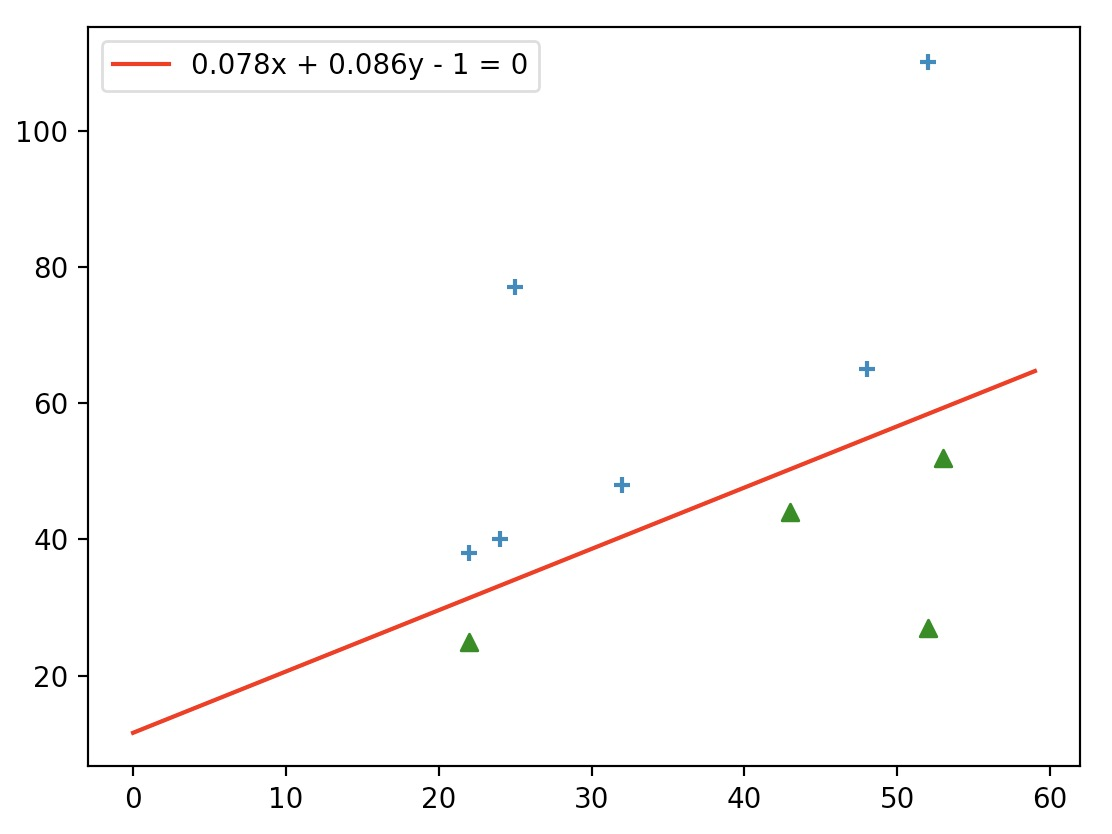
\includegraphics[width=80mm]{./plot.jpg}
	\end{figure*} \\
	对应的决策树为:
	\begin{center}
		\begin{forest}
		[{$0.078x_1 + 0.086x_2\leq 1?$}, draw
			[{0}, ellipse, draw, edge label={node[midway,left,font=\scriptsize]{是}}]
			[{1}, ellipse, draw, edge label={node[midway,right,font=\scriptsize]{否}}]
		]
		\end{forest}
	\end{center}
	此时 $\alpha = -0.078$,$\beta = 0.086$,决策树的深度为 1。
	\vspace{3cm}
	
	
	\section{[25pts] Convolutional Neural Networks}
	\numberwithin{equation}{section}
    \begin{figure*}[h]
    \centering
    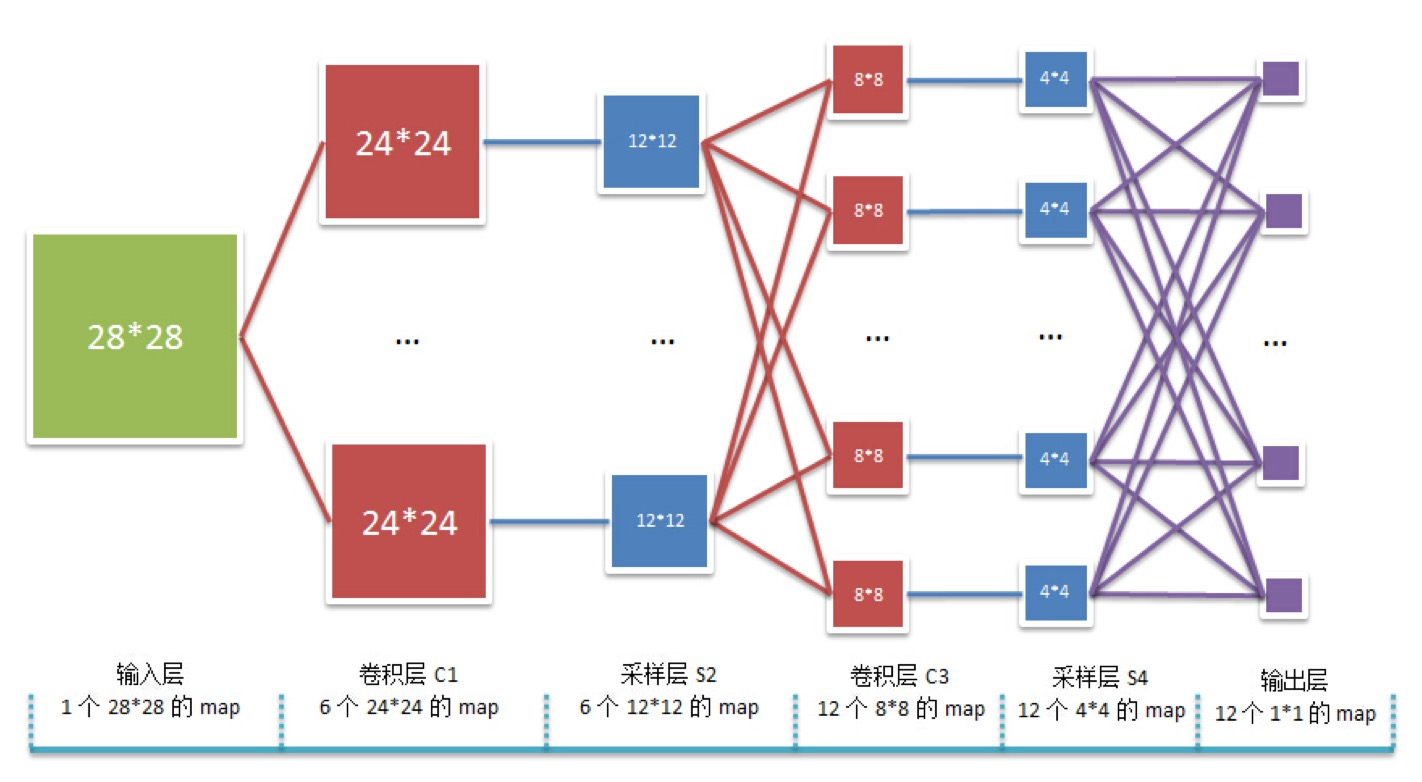
\includegraphics[width=120mm]{./framework.jpg}
   \mbox{ \;\;\;\; ({\it a}) {CNN}}
    \caption{CNN.}\label{fig:f1}
    \end{figure*}
    
    Using Fig. \ref{fig:f1} as an example. Assuming that the loss function of the convolutional neural network is cross-entropy:
    
    \begin{enumerate}
    	\item [(1)] [5 pts] Briefly describe the forward propagation process;
    	\item [(2)] [5 pts] What is the difference between Relu and Sigmoid activation functions;
		\item [(3)] [5 pts] Derivation of the fully connected layer;
   		\item [(4)] [5 pts] Derivation of the pooling layer with average pooling;
    	\item [(5)] [5 pts] Derivation of the convolutional layer with Relu;
    \end{enumerate}
	(1) 输入层通过 6 个含有不同参数的过滤器扫描(过滤器与被扫描区域点乘再加上偏置参数)并经过激活函数形成含有 6 个 map 的卷积层 C1,卷积层的各个 map 经过 2*2 的窗口池化(如平均池化、最大池化等)形成采样层 S2,对采样层的各个 map 进行 12 次卷积运算,并把同一个过滤器得到的卷积结果加和,得到含有 12 个 map 的卷积层 C3,继续对各个卷积层进行采样得到下一个采样层 S4,最后对采样层全连接再通过激活函数(如 Softmax )得到输出层。\\
	(2)	Relu 激活函数保留了非负的输入,把负的输入置为 0,这样相对于 Sigmoid 函数,计算量小,而且由于通过 Relu 函数,一些神经元的输出为 0,保证了网络的稀疏性,缓解了过拟合问题。另一方面,Sigmoid 函数在反向传播时,容易发生梯度消失的情况(当输入的绝对值较大时),从而导致信息丢失,特别是对于深层网络。一般情况下,Relu 激活函数会比 Sigmoid 更有效。\\
	(3) 设某一个样本为 $(X, y)$(其中$y_c = 1$,其余为0),设经过前向传播后得出的分数为 $\hat{y}$,则其交叉熵损失为:
	\begin{equation}
		J = - y_c * \log\hat{y}_c = -\log\hat{y}_c
	\end{equation}
	故输出层的梯度为 $\frac{dJ}{d\hat{y}} = (0, \cdots, 0, -\frac{1}{\hat{y}_c}, 0, \cdots, 0)^T$ 。以图 1 最后一个全连接层为例子,其输入为 12 个 4*4 的矩阵,先将其解开得到一个 192 维的向量(设为 $X_{s_4}$)。设全连接层的参数为 $W$ 和 $b$,则有 $wX_{s_4} + b = \hat{y}$,其中$w$ 为 12*192 的矩阵,$b$ 为 12 维的向量。
	采用链式法则,可得 $w$ 和 $b$ 的梯度为:
	\begin{equation}
	\begin{aligned}
		\frac{dJ}{dw} 
		&= \frac{dJ}{d\hat{y}} * \frac{d\hat{y}}{dw} \\
		&= (0, \cdots, 0, -\frac{1}{\hat{y}_c}, 0, \cdots, 0)^T * X_{s_4} \\
		&= \begin{pmatrix}
			0 & 0 & \cdots & 0 \\ 
			\cdots & \cdots & \cdots & \cdots \\
			0 & 0 & \cdots & 0 \\ 
			-\frac{{X_{s_4}}_{1}}{\hat{y}_c} & -\frac{{X_{s_4}}_{2}}{\hat{y}_c} & \cdots & -\frac{{X_{s_4}}_{192}}{\hat{y}_c}\\
			0 & 0 & \cdots & 0 \\ 
			\cdots & \cdots & \cdots & \cdots \\
			0 & 0 & 0 & 0
			\end{pmatrix} \\ \\
		\frac{dJ}{db}
		&= \frac{dJ}{d\hat{y}} * \frac{d\hat{y}}{db} = (0, \cdots, 0, -\frac{1}{\hat{y}_c}, 0, \cdots, 0)^T
	\end{aligned}
	\end{equation}
	(4) 对于平均池化,其上端梯度会平均分配到对应的池化区域中。如以图 1 倒数第二个池化层为例子,假设池化区域为 2*2,步长为 2,则可知对于池化层 S4 的某一个 8*8 输入 $x$ 及其 4*4 的输出 $y$,有:
	\begin{equation}
		\frac{dJ}{dx_{i,j}} = \frac{dJ}{dy_{\left \lfloor \frac{i+1}{2} \right \rfloor, \left \lfloor \frac{j+1}{2} \right \rfloor}} * \frac{1}{4}
	\end{equation}
	(5) 以图 1 卷积层 C1 为例子,假设每个卷积核 $w_i$ 为 5*5 的矩阵,步长为 1,每个偏置 $b_i$ 为 12*12 的矩阵,同时设卷积层的输入为 $x$, 输出为 $y$,则卷积层的上端梯度为 $\frac{dJ}{dy_{c1}}$(6*12*12 的矩阵)。对其中一个 $w_i$ 进行分析,也即有 $conv({x_{c1}}_i, w_i) + b_i = {y_{c1}}_i$。\\
	对 $w_i$ 中某个位置的数 ${w_i}_{p,q}$ 分析,其扫描过区域为 ${x_i}_{[p\sim(p+23), q\sim(q+23)]}$,故 ${w_i}_{p,q}$ 的梯度为:
	\begin{equation}
		\frac{dJ}{d{w_i}_{p,q}}	= \frac{dJ}{dy_i} * \frac{dy_i}{d{w_i}_{p,q}} = \frac{dJ}{dy_i} · {x_i}_{[p\sim(p+23), q\sim(q+23)]}
	\end{equation}
	对于 $b_i$,其梯度为:
	\begin{equation}
		\frac{dJ}{db_i} = \frac{dJ}{dy_i} * \frac{dy_i}{db_i} = \frac{dJ}{dy_i}
	\end{equation}

	
	\vspace{3cm}
	
	\numberwithin{equation}{section}
	\section{[35 pts] Neural Network in Practice}
	
	In this task, you are asked to build a Convolutional Neural Networks (CNNs) from scratch and examine performance of the network you just build on \textbf{MNIST} dataset.
	Fortunately, there are some out-of-the-box deep learning tools that can help you get started very quickly. For this task, we would like to ask you to work with the \textbf{Pytorch} deep learning framework. Additionally, Pytorch comes with a built-in dataset class for MNIST digit classification task in the \textbf{torchvision} package, including a training set and a validation set. You may find a pytorch introduction at \href{https://pytorch.org/tutorials/beginner/blitz/cifar10_tutorial.html}{here}. Note that, you can use CPU or GPU for training at your choice.
	
	Please find the detailed requirements below.
	
	\begin{enumerate}
		    \item[(1)] [5 pts] You are encouraged to implement the code using \emph{Python3}, implementations in any other programming language will not be judged. Please name the source file (which contains the main function) as \emph{CNN\underline{\hspace{0.5em}}main.py}. Finally, your code needs to print the performance on the provided validation set once executed.
		    
		    \item[(2)] [10 pts] Use any type of CNNs as you want and draw graphs to show your network architecture in the submitted report. You are encouraged to try more architectures.
		    
		    \item [(3)] [15 pts] During training, you may want to try some different optimization algorithms, such as SGD, Adam. Also, you need to study the effect of learning rate and the number of epoch, on the performance (accuracy).
		    
		    \item [(4)] [5 pts] Plot graphs (learning curves) to demonstrate the change of training loss as well as the validation loss during training.
	\end{enumerate}

	\clearpage
	\noindent\textbf{实验报告.}
	\subsection{实验目的与简介}
	本次实验使用 MNIST 数据集和卷积神经网络处理手写数字识别问题,目的是通过卷积神经网络模型,学习手写数字图像特征并进行对新图像的预测。\\
	\indent 本次实验使用 Python3 编程语言及 Pytorch 深度学习框架实现,以下是基本流程图。\\
	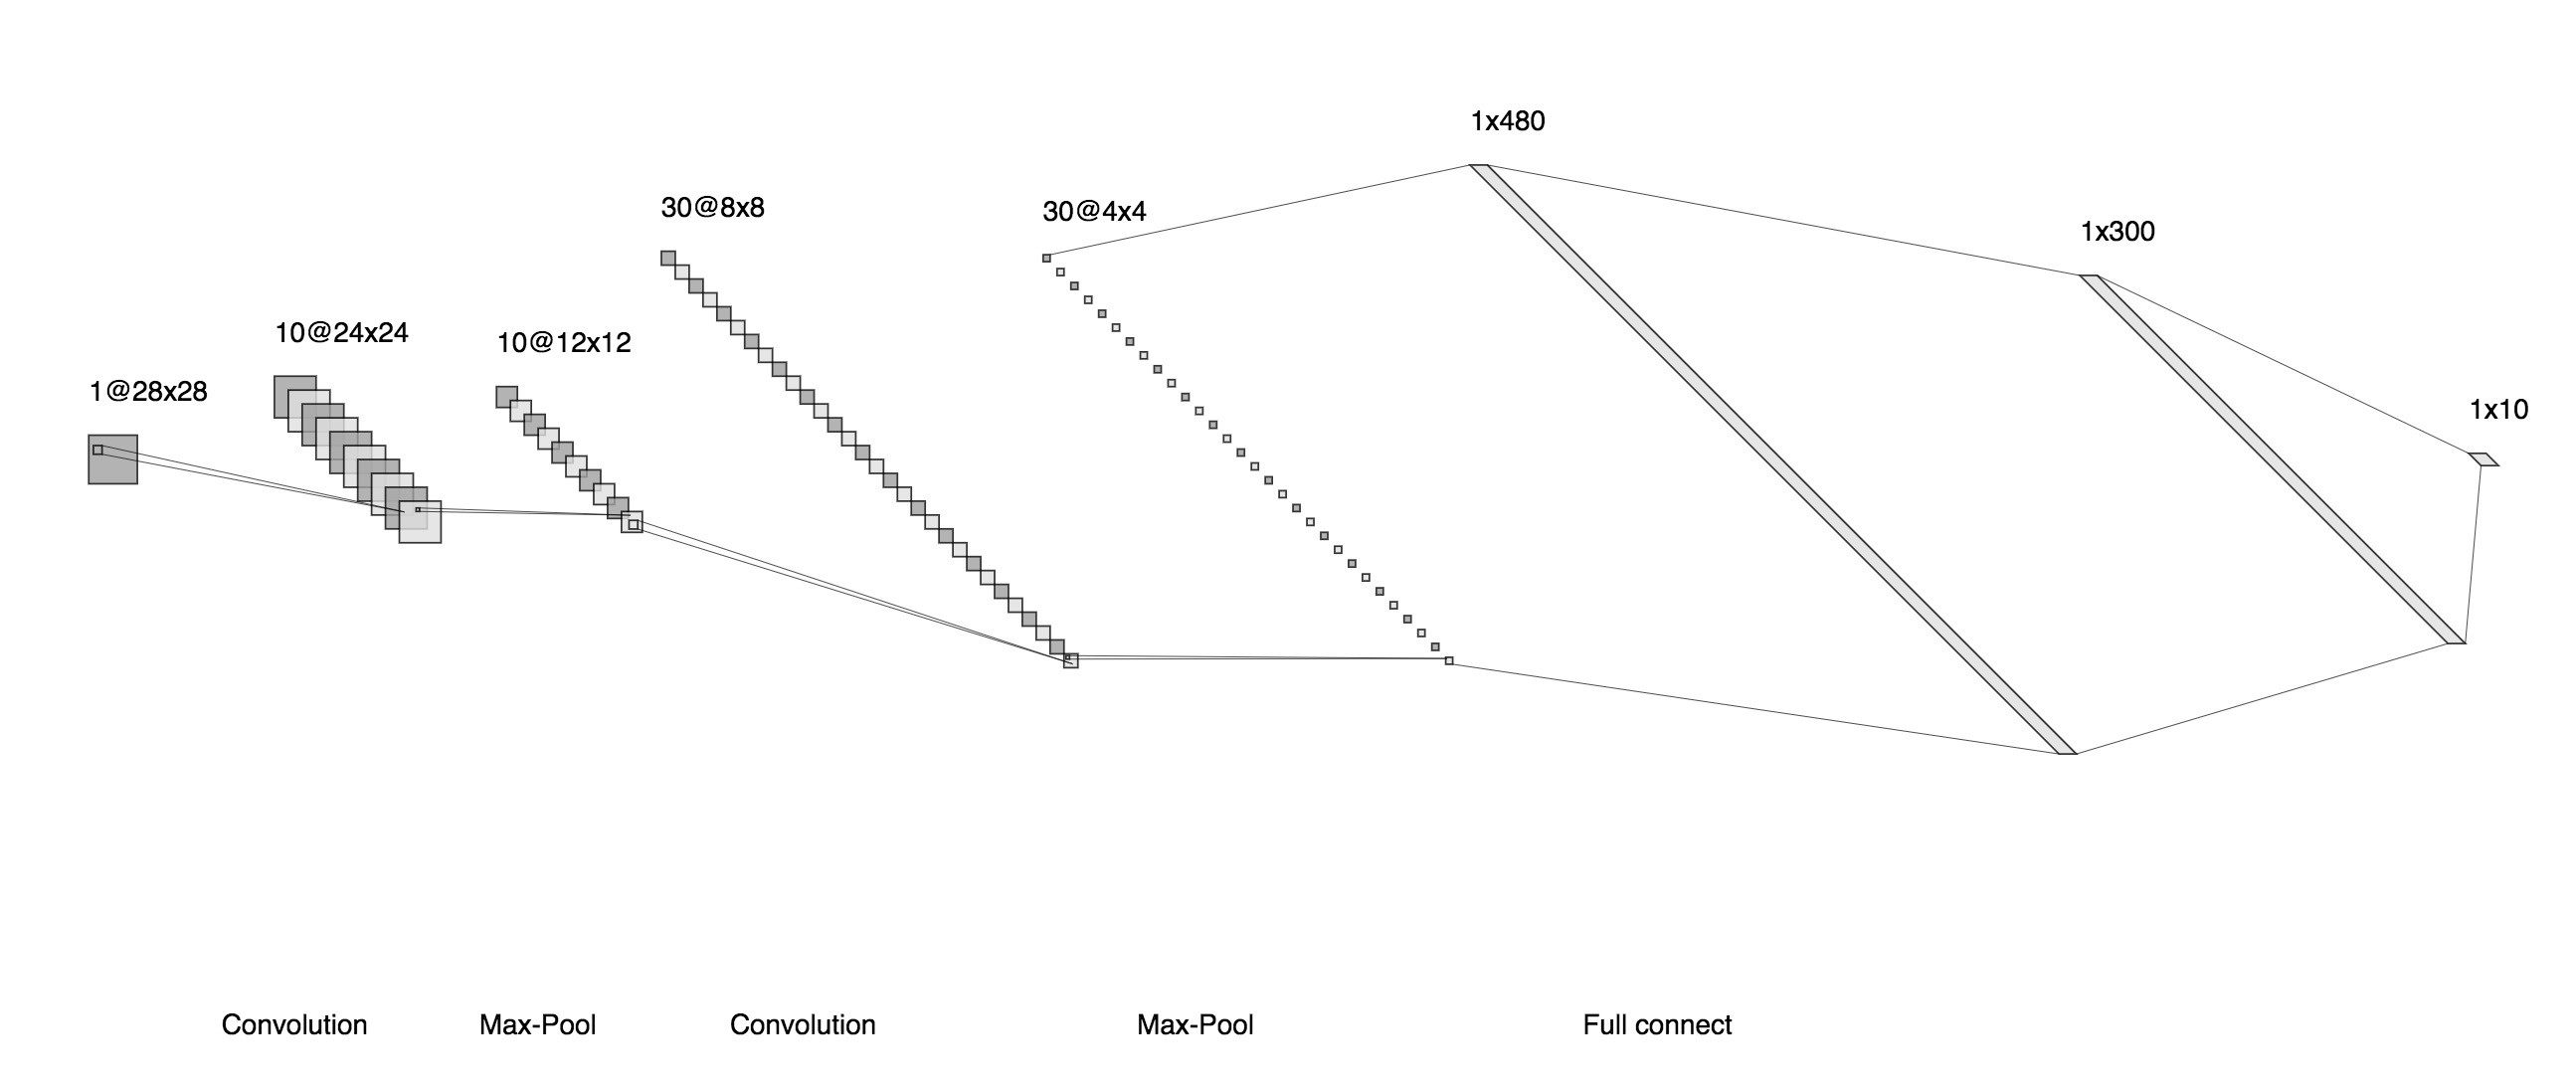
\includegraphics[width = 1.0\textwidth]{nn-architecture.png} \\

	\subsection{数据加载及预处理}
	在加载数据时,将数据进行标准化处理。处理方式为:
	\begin{equation}
		\text{normalize}(x) = \frac{x - \text{mean}}{\text{std}}
	\end{equation}

	\subsection{超参数分析}
	在实验中,我设置调试了以下几个超参数,研究它们对验证结果的影响:\\
	\subsubsection{number of epochs}
	研究数据遍历次数对模型预测性能的影响,可以从对 loss 的分析入手。在 num\_epochs 为 10 的情况下,绘制模型训练过程中的 traning loss 及 validation loss,如下图:\\
	\indent \includegraphics[width = 0.8\textwidth]{loss-epoch10-sdgm-99.png}\\
	\indent 从图中可以看出在 epoch 为 5 时,traning loss 和 validation loss 已经稳定在 0.0 附近。

	\subsubsection{learning rate}
	分别选取 learning rate 为 (0.1, 0.01, 0.001) 分析其对模型预测性能的影响,结果如下:
	\begin{table}[!htbp]
		\centering
		\begin{tabular}{|l|l|l|l|}
		\hline
		learning rate       & 0.1    & 0.01   & 0.001  \\ \hline
		validation accuracy & 95.7\% & 99.2\% & 98.4\% \\ \hline
		\end{tabular}
	\end{table}
	\subsubsection{batch size}
	分别选取 batch size 为 (16, 64, 256) 分析其对模型预测性能的影响,结果如下:
	\begin{table}[htbp]
		\centering
		\begin{tabular}{|l|l|l|l|}
		\hline
		batch size          & 16     & 64     & 256    \\ \hline
		validation accuracy & 98.9\% & 99.2\% & 98.8\% \\ \hline
		\end{tabular}
	\end{table}\\
	\indent 可知 batch size 对模型验证性能影响较小,综合考虑取 64 作为最优选择。
	\subsubsection{optimization method}
	本次实验共考虑了 sgd with momentum, adam 两种优化方法,经过实验两者的收敛速度及验证性能都相当(验证准确率均稍微超过99\%)。
	
	\subsection{最终结果}
	最终考虑超参数组合为:
	\begin{lstlisting}
		num_epochs = 5
		learning_rate = 0.01
		batch_size = 64
		optim_method = 'sgd_momentum' (momentum=0.9)
	\end{lstlisting}
	\quad\quad 训练过程中的训练误差和验证误差变化如下图:\\
	\indent 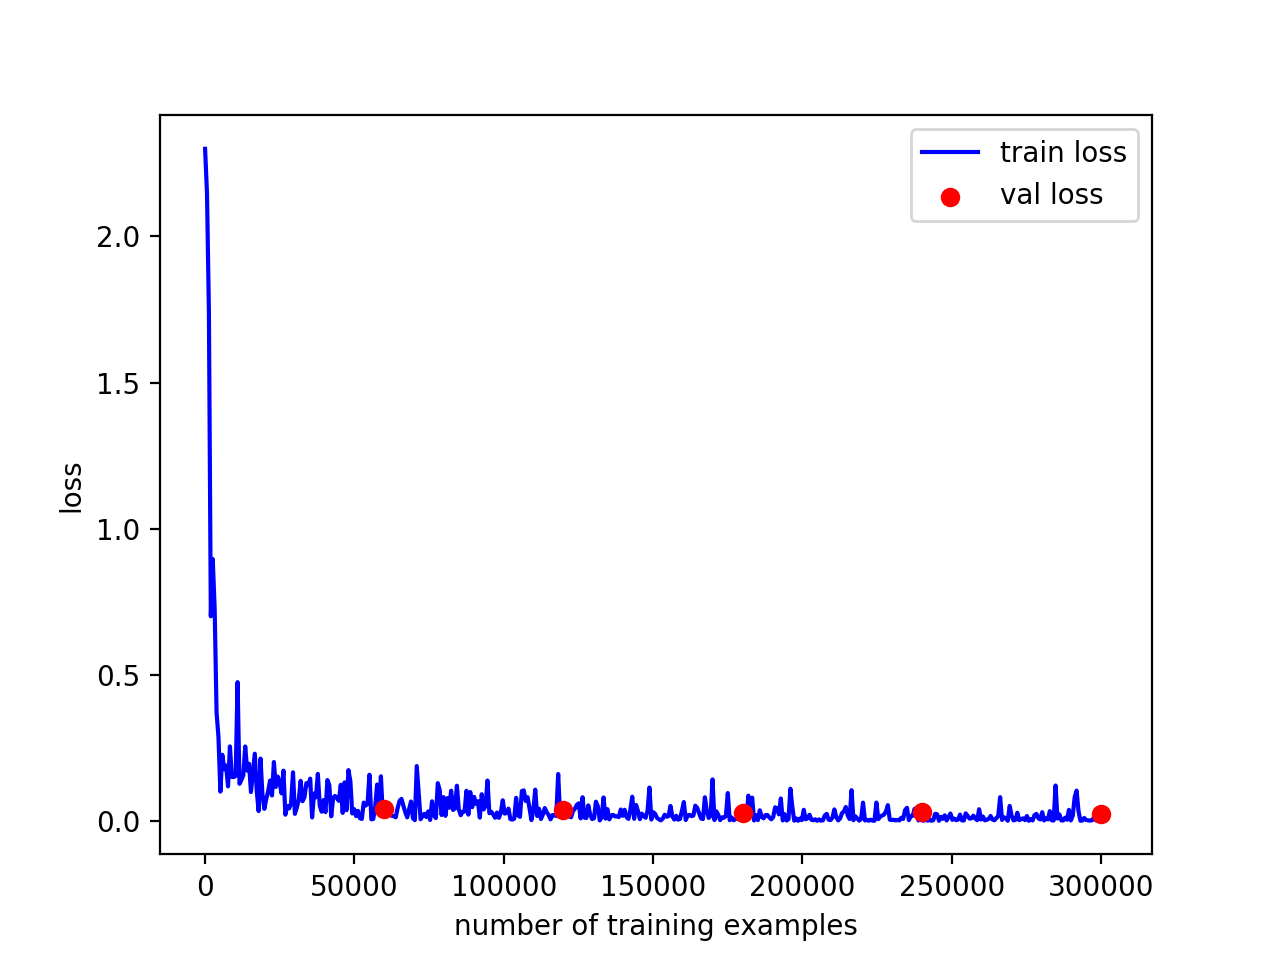
\includegraphics[width = 0.8\textwidth]{loss-result.png}\\
\end{document}
